\documentclass{standalone}
\usepackage{tikz}
\usetikzlibrary{patterns, positioning}


\begin{document}
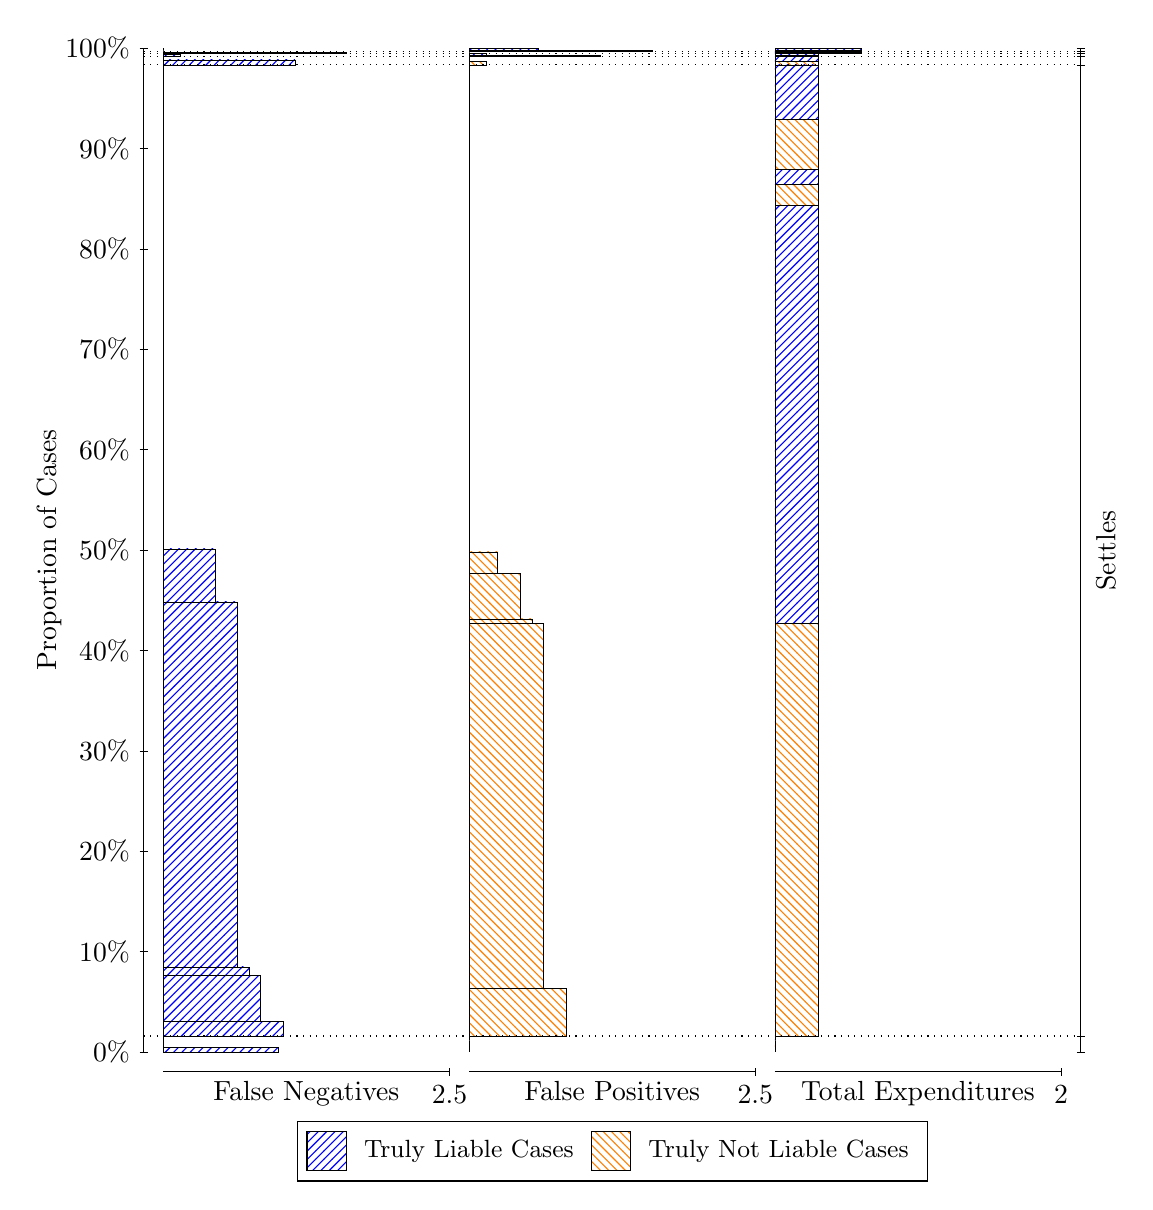
\begin{tikzpicture}
\draw[black, very thin] (1.5,1.75) -- (1.5,14.5);
\node[rotate=90, text=black, anchor=center] at (0.3, 8.125) {Proportion of Cases};
\draw[black, very thin] (1.45,1.75) -- (1.55,1.75);
\node[text=black, anchor=east] at (1.45, 1.75) {0\%};
\draw[black, very thin] (1.45,3.025) -- (1.55,3.025);
\node[text=black, anchor=east] at (1.45, 3.025) {10\%};
\draw[black, very thin] (1.45,4.3) -- (1.55,4.3);
\node[text=black, anchor=east] at (1.45, 4.3) {20\%};
\draw[black, very thin] (1.45,5.575) -- (1.55,5.575);
\node[text=black, anchor=east] at (1.45, 5.575) {30\%};
\draw[black, very thin] (1.45,6.85) -- (1.55,6.85);
\node[text=black, anchor=east] at (1.45, 6.85) {40\%};
\draw[black, very thin] (1.45,8.125) -- (1.55,8.125);
\node[text=black, anchor=east] at (1.45, 8.125) {50\%};
\draw[black, very thin] (1.45,9.4) -- (1.55,9.4);
\node[text=black, anchor=east] at (1.45, 9.4) {60\%};
\draw[black, very thin] (1.45,10.675) -- (1.55,10.675);
\node[text=black, anchor=east] at (1.45, 10.675) {70\%};
\draw[black, very thin] (1.45,11.95) -- (1.55,11.95);
\node[text=black, anchor=east] at (1.45, 11.95) {80\%};
\draw[black, very thin] (1.45,13.225) -- (1.55,13.225);
\node[text=black, anchor=east] at (1.45, 13.225) {90\%};
\draw[black, very thin] (1.45,14.5) -- (1.55,14.5);
\node[text=black, anchor=east] at (1.45, 14.5) {100\%};

\draw[black, very thin] (13.4,1.75) -- (13.4,14.5);
\draw[black, very thin] (13.35,1.75) -- (13.45,1.75);
\node[anchor=west] at (13.35, 1.75) {};
\draw[black, very thin] (13.35,1.9526) -- (13.45,1.9526);
\node[anchor=west] at (13.35, 1.9526) {};
\draw[black, very thin] (13.35,14.287) -- (13.45,14.287);
\node[anchor=west] at (13.35, 14.287) {};
\draw[black, very thin] (13.35,14.395) -- (13.45,14.395);
\node[anchor=west] at (13.35, 14.395) {};
\draw[black, very thin] (13.35,14.428) -- (13.45,14.428);
\node[anchor=west] at (13.35, 14.428) {};
\draw[black, very thin] (13.35,14.459) -- (13.45,14.459);
\node[anchor=west] at (13.35, 14.459) {};
\draw[black, very thin] (13.35,14.5) -- (13.45,14.5);
\node[anchor=west] at (13.35, 14.5) {};

\draw[black, very thin, pattern color=blue, pattern=north east lines] (1.75,1.75) rectangle (3.2033,1.8056);
\draw[black, very thin, pattern color=orange, pattern=north west lines] (1.75,1.8056) rectangle (1.75,1.9526);
\draw[black, very thin, pattern color=blue, pattern=north east lines] (1.75,1.9526) rectangle (3.276,2.1389);
\draw[black, very thin, pattern color=blue, pattern=north east lines] (1.75,2.1389) rectangle (2.9853,2.7185);
\draw[black, very thin, pattern color=blue, pattern=north east lines] (1.75,2.7185) rectangle (2.84,2.8307);
\draw[black, very thin, pattern color=blue, pattern=north east lines] (1.75,2.8307) rectangle (2.6947,7.467);
\draw[black, very thin, pattern color=blue, pattern=north east lines] (1.75,7.467) rectangle (2.404,8.14);
\draw[black, very thin, pattern color=orange, pattern=north west lines] (1.75,8.14) rectangle (1.75,14.287);
\draw[black, very thin, pattern color=blue, pattern=north east lines] (1.75,14.287) rectangle (3.4213,14.349);
\draw[black, very thin, pattern color=orange, pattern=north west lines] (1.75,14.349) rectangle (1.75,14.395);
\draw[black, very thin, pattern color=blue, pattern=north east lines] (1.75,14.395) rectangle (1.968,14.42);
\draw[black, very thin, pattern color=orange, pattern=north west lines] (1.75,14.42) rectangle (1.75,14.428);
\draw[black, very thin, pattern color=blue, pattern=north east lines] (1.75,14.428) rectangle (4.0753,14.443);
\draw[black, very thin, pattern color=orange, pattern=north west lines] (1.75,14.443) rectangle (1.75,14.459);
\draw[black, very thin, pattern color=orange, pattern=north west lines] (1.75,14.459) rectangle (1.75,14.47);
\draw[black, very thin, pattern color=blue, pattern=north east lines] (1.75,14.47) rectangle (1.75,14.5);
\draw[black, very thin, pattern color=orange, pattern=north west lines] (5.6333,1.75) rectangle (5.6333,1.897);
\draw[black, very thin, pattern color=blue, pattern=north east lines] (5.6333,1.897) rectangle (5.6333,1.9526);
\draw[black, very thin, pattern color=orange, pattern=north west lines] (5.6333,1.9526) rectangle (6.8687,2.5549);
\draw[black, very thin, pattern color=orange, pattern=north west lines] (5.6333,2.5549) rectangle (6.578,7.1913);
\draw[black, very thin, pattern color=orange, pattern=north west lines] (5.6333,7.1913) rectangle (6.4327,7.2489);
\draw[black, very thin, pattern color=orange, pattern=north west lines] (5.6333,7.2489) rectangle (6.2873,7.8285);
\draw[black, very thin, pattern color=orange, pattern=north west lines] (5.6333,7.8285) rectangle (5.9967,8.1001);
\draw[black, very thin, pattern color=blue, pattern=north east lines] (5.6333,8.1001) rectangle (5.6333,14.287);
\draw[black, very thin, pattern color=orange, pattern=north west lines] (5.6333,14.287) rectangle (5.8513,14.334);
\draw[black, very thin, pattern color=blue, pattern=north east lines] (5.6333,14.334) rectangle (5.6333,14.395);
\draw[black, very thin, pattern color=orange, pattern=north west lines] (5.6333,14.395) rectangle (7.3047,14.403);
\draw[black, very thin, pattern color=blue, pattern=north east lines] (5.6333,14.403) rectangle (5.8513,14.428);
\draw[black, very thin, pattern color=orange, pattern=north west lines] (5.6333,14.428) rectangle (5.6333,14.443);
\draw[black, very thin, pattern color=blue, pattern=north east lines] (5.6333,14.443) rectangle (5.6333,14.459);
\draw[black, very thin, pattern color=orange, pattern=north west lines] (5.6333,14.459) rectangle (7.9587,14.47);
\draw[black, very thin, pattern color=blue, pattern=north east lines] (5.6333,14.47) rectangle (6.5053,14.5);
\draw[black, very thin, pattern color=orange, pattern=north west lines] (9.5167,1.75) rectangle (9.5167,1.897);
\draw[black, very thin, pattern color=blue, pattern=north east lines] (9.5167,1.897) rectangle (9.5167,1.9526);
\draw[black, very thin, pattern color=orange, pattern=north west lines] (9.5167,1.9526) rectangle (10.062,7.1913);
\draw[black, very thin, pattern color=blue, pattern=north east lines] (9.5167,7.1913) rectangle (10.062,12.501);
\draw[black, very thin, pattern color=orange, pattern=north west lines] (9.5167,12.501) rectangle (10.062,12.772);
\draw[black, very thin, pattern color=blue, pattern=north east lines] (9.5167,12.772) rectangle (10.062,12.959);
\draw[black, very thin, pattern color=orange, pattern=north west lines] (9.5167,12.959) rectangle (10.062,13.596);
\draw[black, very thin, pattern color=blue, pattern=north east lines] (9.5167,13.596) rectangle (10.062,14.287);
\draw[black, very thin, pattern color=orange, pattern=north west lines] (9.5167,14.287) rectangle (10.062,14.334);
\draw[black, very thin, pattern color=blue, pattern=north east lines] (9.5167,14.334) rectangle (10.062,14.395);
\draw[black, very thin, pattern color=orange, pattern=north west lines] (9.5167,14.395) rectangle (10.062,14.403);
\draw[black, very thin, pattern color=blue, pattern=north east lines] (9.5167,14.403) rectangle (10.062,14.428);
\draw[black, very thin, pattern color=orange, pattern=north west lines] (9.5167,14.428) rectangle (10.607,14.443);
\draw[black, very thin, pattern color=blue, pattern=north east lines] (9.5167,14.443) rectangle (10.607,14.459);
\draw[black, very thin, pattern color=orange, pattern=north west lines] (9.5167,14.459) rectangle (10.607,14.47);
\draw[black, very thin, pattern color=blue, pattern=north east lines] (9.5167,14.47) rectangle (10.607,14.5);
\draw[black, dotted] (1.5,1.9526) -- (13.4,1.9526);
\draw[black, dotted] (1.5,14.287) -- (13.4,14.287);
\draw[black, dotted] (1.5,14.395) -- (13.4,14.395);
\draw[black, dotted] (1.5,14.428) -- (13.4,14.428);
\draw[black, dotted] (1.5,14.459) -- (13.4,14.459);
\draw[black, very thin] (1.75,1.5) -- (5.3833,1.5);
\node[text=black, anchor=north] at (3.5667, 1.5) {False Negatives};
\draw[black, very thin] (5.3833,1.45) -- (5.3833,1.55);
\node[text=black, anchor=north] at (5.3833, 1.45) {2.5};

\draw[black, very thin] (5.6333,1.5) -- (9.2667,1.5);
\node[text=black, anchor=north] at (7.45, 1.5) {False Positives};
\draw[black, very thin] (9.2667,1.45) -- (9.2667,1.55);
\node[text=black, anchor=north] at (9.2667, 1.45) {2.5};

\draw[black, very thin] (9.5167,1.5) -- (13.15,1.5);
\node[text=black, anchor=north] at (11.333, 1.5) {Total Expenditures};
\draw[black, very thin] (13.15,1.45) -- (13.15,1.55);
\node[text=black, anchor=north] at (13.15, 1.45) {2};


\node[text=black, centered, rotate=90] at (13.72, 8.1201) {Settles};





\draw (7.449999999999999,1.5) node[draw=none] (baseCoordinate) {};
\begin{scope}[align=center]
        \matrix[scale=0.5, draw=black, below=0.5cm of baseCoordinate, nodes={draw}, column sep=0.1cm]{
            \node[rectangle, draw, minimum width=0.5cm, minimum height=0.5cm, pattern color=blue, pattern=north east lines] {}; &
            \node[draw=none, font=\small, text=black] (B) {Truly Liable Cases}; &
            \node[rectangle, draw, minimum width=0.5cm, minimum height=0.5cm, pattern color=orange, pattern=north west lines] {}; &
            \node[draw=none, font=\small, text=black] (B) {Truly Not Liable Cases}; \\
            };
\end{scope}

\end{tikzpicture}
\end{document}